\documentclass{beamer}
\usepackage[utf8]{inputenc}
\usepackage[russian]{babel}
\usepackage[T2A]{fontenc}
\usepackage{amsmath}
\usepackage{amsfonts}
\usepackage{amsthm}
\usepackage{bbm}
\usepackage{amssymb}
\usepackage{bm}
\usepackage{graphicx}
\usepackage{epstopdf}
\usepackage[]{algorithm2e}
\usepackage{amsthm}

%\usetheme{Warsaw}
%\usecolortheme{sidebartab}
\usetheme{Warsaw}
\usecolortheme{seahorse}

%\definecolor{beamer@blendedblue}{RGB}{255,255,0}
%\definecolor{beamer@blendedblue}{HTML}{008A34} %green
%\definecolor{beamer@blendedblue}{HTML}{4A4A4A} %grey
%\definecolor{beamer@blendedblue}{HTML}{0E9059} %biryuz
\definecolor{beamer@blendedblue}{HTML}{027466} %blue


\theoremstyle{definition}
\newtheorem{defin}{Definition}
\newtheorem{assumption}{Assumption}
\theoremstyle{plain}
\newtheorem{thm}{Theorem}
\newtheorem{lem}{Lemma}
\newtheorem{prop}{Proposition}
\theoremstyle{remark}
\newtheorem{remark}{Remark}
\newtheorem{prob}{Problem}
\def\eqdef{\stackrel{def}{=}}

% \DeclareMathOperator*{\argmin}{argmin}
% \DeclareMathOperator*{\Argmin}{Argmin}
% \DeclareMathOperator{\barcnt}{bar}
% \DeclareMathOperator{\supp}{supp}
% \DeclareMathOperator{\est}{\mathbb{E}}
% \DeclareMathOperator{\inter}{int}
% \DeclareMathOperator{\ind}{Ind}

\begin{document}
\setlength{\abovedisplayskip}{5pt}
\setlength{\belowdisplayskip}{5pt}

	\title[\hbox to 60mm{Optimization approaches to community detection \hfill\insertframenumber\,/\,15}]
			{ Course project \\ <<Optimization approaches to community detection>>}
	\author[M. Danilova, A. Podkopaev, N. Puchkin, I. Silin]{\large Marina Danilova, Alexander Podkopaev, Nikita Puchkin, Igor Silin}
	\institute[Affiiation]{
	\textsc{Skolkovo institute of science and technology}
	}

\date{\footnotesize{December 16, 2016}}

	\begin{frame}
		\titlepage
	\end{frame}

	\begin{frame}{Plan}
		  \tableofcontents[
		    sectionstyle=show/show,
		    subsectionstyle=show/show/show
		  ]
	\end{frame}

		% \AtBeginSection[]
		% {
		%   \begin{frame}{Plan of the following section}
		%   \tableofcontents[
		%     currentsection,
		%     sectionstyle=show/shaded,
		%     subsectionstyle=show/show/shaded
		%   ]
		%   \end{frame}
		% }
	
	\section{Introduction to community detection}

			\begin{frame}{Example}
				\vspace{-17pt}
				\center{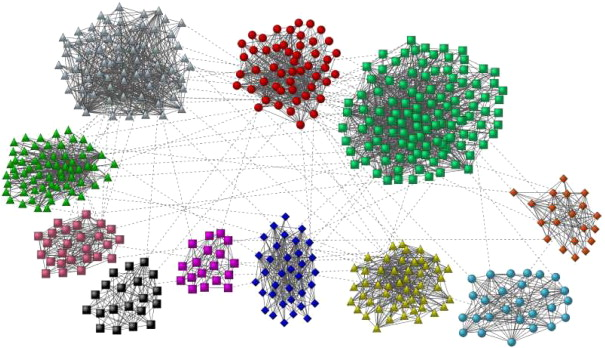
\includegraphics[width=0.9\linewidth]{Images//communities.png}}
				\\
				The goal of community detection is to find \textbf{partition} of nodes into \textbf{non-overlapping} clusters.
			\end{frame}
		
			\begin{frame}{Notations}

			\vspace{-5pt}
			\begin{block}{Graph}
				\begin{itemize}
					\item \textbf{Undirected unweighted} graphs \textbf{without loops} with $n$ nodes and $m$ edges.
					\item The nodes are enumerated as $\{ 1, ..., n\}$.\\
					\item Graph is given by its $n \times n $ adjacency matrix $A$.
					\item Degree of the node $i$ is $d_i$.
				\end{itemize}

			\end{block}

			\vspace{-5pt}
			\begin{block}{Clusters}
				\begin{itemize}
				\item The number of clusters is $k$.\\
				\item The clusters are denoted as $\mathcal{C}_1, ..., \mathcal{C}_k$.
				\item Cluster sizes are $ |\mathcal{C}_1|, ..., |\mathcal{C}_k|$.
				\item Labeling $z$: $z(i)$ is the cluster containing node $i$, i.e. $i \in \mathcal{C}_{z(i)}$.
				\end{itemize}
			\end{block}
		\end{frame}

	\section{Algorithms}

		\subsection{Modularity-based method}
			\begin{frame}{Modularity-based method}
				\vspace{-5pt}
				\begin{block}{Modularity}
					\begin{itemize}
						\item Fraction of edges which lie within communities:
								\begin{equation}
									\begin{aligned}
										\frac{1}{2m} \sum\limits_{i,j=1}^{n} a_{ij} \cdot \mathbbm{1}\{ z(i) = z(j) \}.
										\nonumber
									\end{aligned}
								\end{equation}
						\item Expected fraction of edges which lie within communities (for some probabilistic model):
								\begin{equation}
									\begin{aligned}
										\sum\limits_{i,j=1}^{n}\frac{d_i}{2m}\frac{d_j}{2m} \cdot \mathbbm{1}\{ z(i) = z(j) \}.
										\nonumber
									\end{aligned}
								\end{equation}
						\item \textbf{Modularity} is the difference between two previous fractions:
								\begin{equation}
									\begin{aligned}
										Q(z) =
										\frac{1}{2m} \sum\limits_{i,j=1}^{n} \left(a_{ij} - \frac{d_i\cdot d_j}{2m}\right) \cdot \mathbbm{1}\{ z(i) = z(j) \}.
										\nonumber
									\end{aligned}
								\end{equation}
					\end{itemize}
				\end{block}
			\end{frame}

			\begin{frame}{Modularity-based method}
			\vspace{-5pt}
				\begin{block}{Formulating an optimization problem}
					\begin{equation}
						\begin{aligned}
							&maximize\;\;Q\\
							&s.t. \text{ all possible labelings }z
						\nonumber
						\end{aligned}
					\end{equation}
				\end{block}

				\begin{block}{Greedy algorithm}
						1. Initially every node forms its own cluster: $\mathcal{C}_i = \{ i \}$ and $Q = 0$.\\
						2. Iteratively:
							\begin{itemize}
								\item choose two current clusters, joining of which gives maximal gain $\Delta Q$ of modularity.
								\item unite these two current clusters into one and recalculate $Q := Q + \Delta Q$.
							\end{itemize}
						3. Pick the clustering with maximal $Q$ from partitions that we had during the iterations.
				\end{block}
			\end{frame}

		\subsection{Spectral method}
			\begin{frame}{Spectral method}
				\begin{block}{Measuring sizes of clusters}
					Consider the following two ways of measuring size of clusters:
					\begin{itemize}
						\item $|\mathcal{C}_{i}| = \{\text{number of vertices in $\mathcal{C}_{i}$}\}$
						\item $vol(\mathcal{C}_{i}) = \sum \limits_{i \in \mathcal{C}_{i}}d_{i}$
					\end{itemize}
				\end{block}
				\begin{block}{MinCut}
					Define $W(\mathcal{C}_p,\mathcal{C}_q):= \sum \limits_{i \in \mathcal{C}_p,j \in C_q}  a_{ij}.$ Then MinCut problem is:
\[
cut(\mathcal{C}_1,\dots,\mathcal{C}_k) = \frac{1}{2}\sum\limits_{i=1}^kW(\mathcal{C}_i,\overline{\mathcal{C}_i}) \rightarrow \min \limits_{\mathcal{C}_1,\dots,\mathcal{C}_k}
\]
				\end{block}
			\end{frame}		
		\begin{frame}{Spectral method}
				\begin{block}{RatioCut and Normalized Cut}
					The MinCut solution separates one individual vertex from the rest. The following objectives are considered:
\[
RatioCut(\mathcal{C}_1,\dots,\mathcal{C}_k) = \sum \limits_{i=1}^k \frac{cut(\mathcal{C}_i,\overline{\mathcal{C}_i})}{|\mathcal{C}_{i}|} \rightarrow \min \limits_{\mathcal{C}_1,\dots,\mathcal{C}_k}
\]

\[
NormCut(\mathcal{C}_1,\dots,\mathcal{C}_k)= \sum \limits_{i=1}^k \frac{cut(\mathcal{C}_i,\overline{\mathcal{C}_i})}{vol(\mathcal{C}_{i})} \rightarrow \min \limits_{\mathcal{C}_1,\dots,\mathcal{C}_k}
\]
			\end{block}
				Balancing conditions lead to NP-hard problem. Spectral clustering is a way to solve relaxed versions of those problems
			\end{frame}
		 	\begin{frame}{Spectral method}
				\begin{block}{Types of Laplacians}
					\begin{itemize}
						\item Unnormilized Laplacian: $L=D-A$
						\item Symmetric Laplacian: $L_{sym} =D^{-\frac{1}{2}}LD^{-\frac{1}{2}}=I-D^{-\frac{1}{2}}AD^{-\frac{1}{2}}$
						\item Random walk Laplacian: $L_{rw} =D^{-1}L=I-D^{-1}A$
					\end{itemize}
				\end{block}

				\begin{block}{Idea}
					\begin{itemize}
						\item Solving relaxed problem is equivalent to considering eigenvectors corresponding to $k$ smallest eigenvalues of Laplacian that describe cluster properties of given graph
					\end{itemize}
				\end{block}
				
			\end{frame}	
		
		\subsection{Semidefinite relaxation method}
			\begin{frame}{Semidefinite relaxation method}
				\begin{block}{Clustering matrix}
				\begin{itemize}
					\item Clustering matrix $X$ of size $n\times n$ with $x_{ij} = \mathbbm{1}\{ z(i) = z(j) \}$.\\
					\item Space of all matices with such structure is $\mathcal{X}$.
				\end{itemize}
				\end{block}
				
				\begin{block}{Formulating an optimization problem}
				Likelihood for special case of stochstic block model is
				\begin{equation}
					\begin{aligned}
						\mathcal{L}(X) = trace(AX).
					\nonumber
					\end{aligned}
				\end{equation}
				Maximum likelihood method:
				\begin{equation}
					\begin{aligned}
						&maximize\;\;\mathcal{L}(X)\\
						&s.t. \;\;X \in \mathcal{X}
					\nonumber
					\end{aligned}
				\end{equation}
				NP-hard combinatorial optimization problem $\Rightarrow$ relaxations!
				\end{block}
			\end{frame}

			\begin{frame}{Semidefinite relaxation method}
				\begin{block}{Semidefinite relaxation}
				We just relax $X \in \mathcal{X}$ and get semidefinite program:
				\begin{equation}
					\begin{aligned}
						&maximize\;\;trace(AX)\\
						&s.t. \;\;X \text{ is positive semi-definite}, \\
						&\;\;\;\;\;\;\; X \geq 0, \\
						&\;\;\;\;\;\;\; diagonal(X) = e, \\
						&\;\;\;\;\;\;\; Xe = \frac{n}{k}e,
					\nonumber
					\end{aligned}
				\end{equation}
				where $e = (1,\ldots,1)^T$.\\
				\vspace{5pt}
				This problem can be solved with SDP solvers implemented in cvx.
				\end{block}
			\end{frame}


		\subsection{Natural conjugate gradients method}
			\begin{frame}{Natural conjugate gradients method} %{Conjugate gradients method}
                \begin{itemize}
                    \item Model parametrized by
                        \begin{equation}
                            \begin{aligned}
                            \nonumber
                                & z(i) \sim \text{Poly}(\pi), \quad i=\overline{1, n} \\
                                & P = \| p_{ij} \|_{i,j=\overline{1,k}} \text{ - probabilities of inter-cluster edges occurrence} \\
                            \end{aligned}
                        \end{equation}

                    \item Bayesian approach:
                    \begin{equation}
                        \begin{aligned}
                        \nonumber
                            & \pi \sim \text{Dirichlet}(\alpha) \\
                            & p_{ii} \sim \text{Beta}(\beta), \quad i = \overline{1,k} \\
                            & p_{ij} \ll 1, \quad \forall i\neq j
                        \end{aligned}
                    \end{equation}
                    \item $p(z, \pi, P | A)$ - true posterior with observed adjacency matrix $A$
                    \item $\mathcal Q$ - family of feasible distributions
                \end{itemize}

			\end{frame}

			\begin{frame}{Natural conjugate gradients method} %{Conjugate gradients method}
				\begin{block}{Formulating an optimization problem}
                    \begin{equation*}
                        \mathcal L(q) \equiv -\text{KL}\left(q \| p(Z, \pi, P | A)\right) \longrightarrow \max\limits_{q \in \mathcal Q}
                    \end{equation*}
				\end{block}
                \begin{itemize}
				    \item The problem can be reduced to unconstrained optimization:

                        \begin{equation}
                            \begin{aligned}
                            \nonumber
                            \mathcal L = \mathcal L(\theta) \longrightarrow \max, \quad \text{$\theta$ - $n\times(k-1)$ matrix}
                            \end{aligned}
                        \end{equation}

                    \item Use conjugate gradients method in a statistical manifold
                    \item Metrics is defined by a matrix
                        \[
                            \mathcal I(\theta) - \text{Fischer information}
                        \]
                \end{itemize}
			\end{frame}

	\section{Experimental results}
		\begin{frame}{}
		\centering{Artificial graph:}
			\begin{columns}
					\column{0.5\textwidth}
						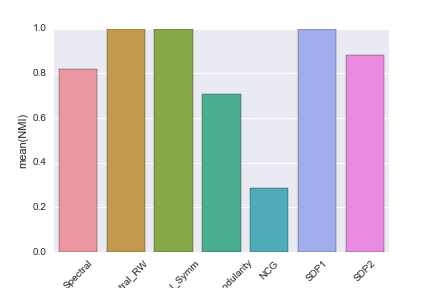
\includegraphics[width=0.9\linewidth]{Images/sbm_NMI.png}
					\column{0.5\textwidth}
						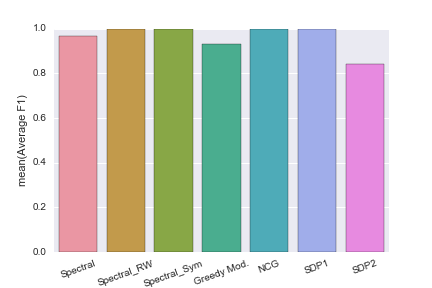
\includegraphics[width=0.9\linewidth]{Images/sbm_AverageF1.png}
				\end{columns}
		\centering{Real-world graph:}
			\begin{columns}
					\column{0.5\textwidth}
						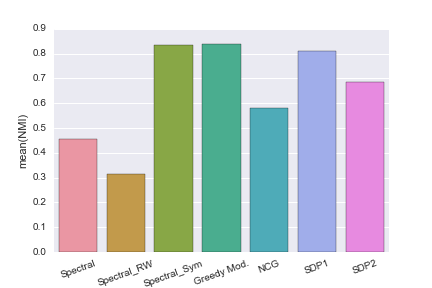
\includegraphics[width=0.9\linewidth]{Images/karate_NMI.png}
					\column{0.5\textwidth}
						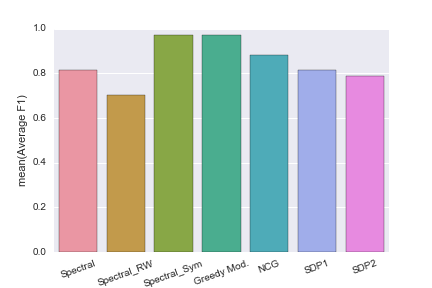
\includegraphics[width=0.9\linewidth]{Images/karate_AverageF1.png}
				\end{columns}
				
		\end{frame}


	\section*{}

		\begin{frame}{}
			\centering{ \LARGE Thanks for your attention!}
		\end{frame}

\end{document} 